\section{Selective identification of IP devices} \label{sec:method}
The main goal of this project is to propose methods to identify devices that fulfill within the following constraints:
\begin{itemize}
    \item The device is connected to the internet 
    \item The device is part of a Cyber Physical System(CPS)
    \item The device is part of either the maritime or offshore industries
\end{itemize}
As all the work is done online, the first constraint will always be fulfilled using the workflow of this project. 
Then several methods to filter devices based on industry is suggested in \cref{sec:identify_industry}. These methods are not exclusive, and multiple methods may for example be used to double-check the validity of the results.
From these results, the CPS should be separated. This is explained in \cref{sec:identify_cps}.

\subsection{Identifying devices from spesific industries} \label{sec:identify_industry}
\subsubsection{Banner similarities} \label{sec:banner_method}
When connecting a device to the internet, it needs to be configured. The installer needs competence to do this properly, and to spend time to perform the installation. To make such devices more accessible and efficient, finished solutions are most often used. Due to this, the same devices mostly have the same default configuration, and therefore the same banners. This can be used to identify devices within the chosen constraints by using the following method.
\begin{enumerate}
    \item Choose a device type that fulfill the constraints and may be connected to the internet.
    \item Find the IP address of one instance of such a device, and find its Shodan entry.
    \item Get its banner.
    \item Use unique information from the banner to find all devices with similar banners.
\end{enumerate}
The most difficult of these steps is to find the IP address. The easiest way to do this is to own a device and find its IP address. Unfortunately, this project does not have access to any devices that fit the constraints set.
If this is not an option, the device could be found by guessing what information could be found in its banner, for example the device name or ports it has open.


\subsubsection{Internet Service Provider and IP ranges} \label{sec:isp_method}
Internet Service Providers(ISP) are the organizations that connect people and companies to the internet. ISPs charge money to deliver internet connectivity, and most people have a subscription. Telenor is for example a Norwegian ISP. While a lot of ISPs are generalized, and deliver the internet to both private and organizational customers, others can be more specialized. 

Regional Internet Registries (RIR) sell IP addresses to organizations, for them to distribute further. For example, an Internet Service Provider(ISP) will buy an CIDR range, then give IPv4 addresses to the customers while they use their subscribed internet connections. An overview of the distribution of IPv4 addresses to organizations is illustrated in \cref{fig:ipv4_map}. Shodan can use the filter "isp" to search for ISPs, "org" to search for organizations, and "net" to search for devices in a CIDR range. 

\begin{figure} [H]
    \centering
    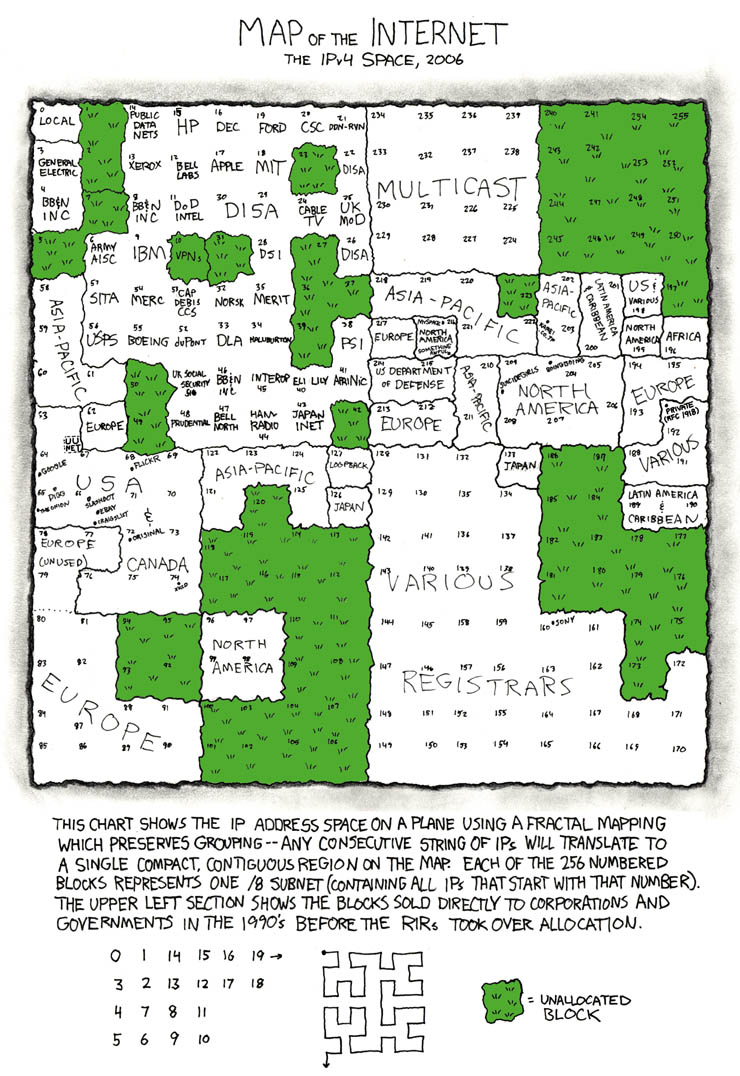
\includegraphics[scale=4]{Figurer/map_of_the_internet.jpg}
    \caption{A map of the IPv4 space, from the XKCD web comic. \cite{xkcd} }
    \label{fig:ipv4_map}
\end{figure}

While it is straight forward to find the name of an organization or ISP, a tool is needed to find CIDR ranges. One or more CIDR range that is owned by an organization and has a single defined routing policy is called an Autonomous System(AS). A typical example of an organization that owns an AS, is an Internet Service Provider(ISP). \cite{AS_def} 
The AS are registered with unique identification numbers. Online tools, like \href{https://hackertarget.com/as-ip-lookup/}{\textbf{Hackertarget AS-IP lookup}} \cite{asip_lookup}, makes it possible to find the parent AS of an IP address. Then the rest of the IP addresses belonging to the same AS can be found.


\subsubsection{Reverse IP geolocation} \label{sec:geo_method}
When Regional Internet Registries (RIR) give IP addresses to organizations, they also register contact information on the IP addresses. A part of this information is a location, specifying a country and city. Some data providers claim that the country accuracy is between 95\% and 99\%, while the city accuracy is between 50\% and 75\%.\cite{geolocation_acc}With accuracy that poor, it is not possible to decide if an IP address is within the constraints by using IP geolocation. The information returned by the one of the RIRs can be seen in \cref{fig:RIPE_NCC}.
Shodan have a filter for the location. This filter can also filter by latitude and longitude. However, I have not been able to find any information on how Shodan gather this information. \todo{Er det innafor å seie "I have" her?} 
Because of these uncertainties, IP geolocation can not be conclusive for finding devices within the constraints. However, by reversing the technique, it would be possible to narrow down the selection of IP addresses by first defining an area. Shodan can use the filter "geo:latitude,longitude,radius" to filter on addresses based on location.  

\begin{figure} [H]
    \centering
    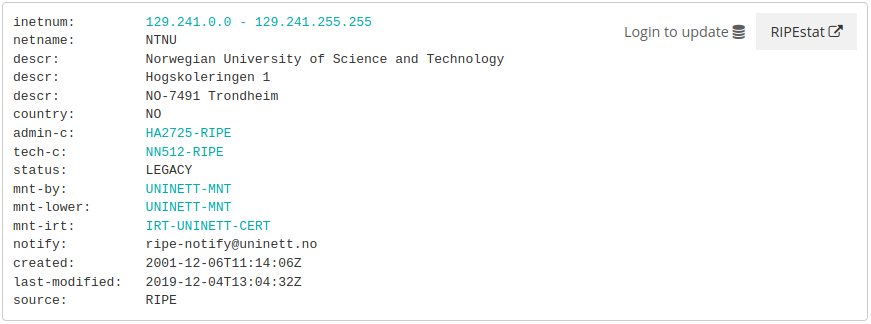
\includegraphics[scale=0.5]{Figurer/ripe.png}
    \caption{The IP address lookup of RIPE NCC \cite{ripe_whois}}
    \label{fig:RIPE_NCC}
\end{figure}

\subsubsection{Latency and traceroute}
The simplest form of reaching another device on the internet is called a "ping". This sends a echo request to an IP address, to make it send a response back. It is mostly used to check if a device is reachable. To prevent a bug where packets travel in an infinite loop instead of reaching the recipient, packets have a Time To Live (TTL) counter. This counter increments every time a packet travels trough a switch or router. When this counter is reached, the packet is stopped, and a message is returned to the sender, informing it of the loss.
The "traceroute" command takes advantage of the fact that the Time To Live counter can be set by the sender. It will start the TTL counter at 1 and sending a message towards a predefined target IP address. This message will then travel 1 step towards its target before it is returned. Then it increments this counter and repeats the send. This way, all routers the packet travel trough on its way will be indexed. In addition, traceroute will time how long the packet uses before it is returned, called "Round Trip Time"(RTT).
The Round Trip Time can give an idea of how the signal travels. Faster RTT can be because of shorter distance or better infrastructure. On the other hand, slow RTT can indicate farther distance or worse infrastructure.
The tracroute is visualized in \cref{fig:latency}. Here the signal will travel fast from Source to both Router 1 and Router 2. There will then be a jump in latency when the signal crosses the atlantic ocean on its way to router 3. The longest delay will be where the signal travels to the Destination from Router 3 trough a satellite.

\begin{figure} [H]
    \centering
    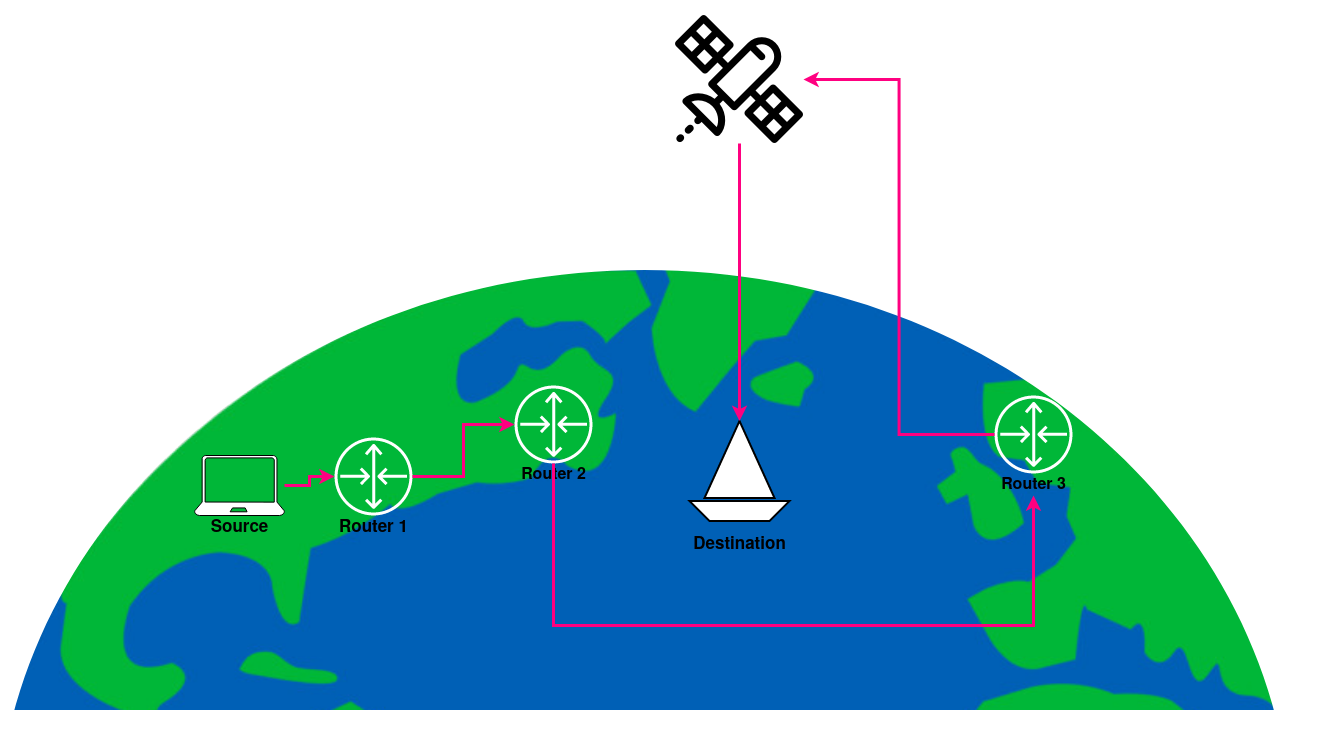
\includegraphics[scale=0.3]{Figurer/latency.png}
    \caption{Visualization of internet latency. Map from \href{http://getdrawings.com/earth-cartoon-drawing}{http://getdrawings.com/earth-cartoon-drawing}}
    \label{fig:latency}
\end{figure}

\subsection{Identifying devices from Cyber-Physical Systems} \label{sec:identify_cps}
As mentioned in \cref{sec:cps}, Cyber-Physical Systems(CPS) is a system containing anything from real-time controllers to human operators. Not all CPS have components that are connected to the internet. When a CPS is connected to the internet, only some of its components are actually connected. In the offshore industry, CPS are typically Industrial Control Systems(ICS). In the maritime industy, CPS are typically navigation systems. As these industries often overlap, their CPS usecases often overlap as well. Approaches for identifying two subsections of CPS, ICS and navigation systems will be proposed below.

\subsubsection{Industrial Control Systems}
Industrial Control Systems(ICS) are mostly easy to identify. A lot of previous research already exist on Shodan and ICS. For example: \textit{Exploring Shodan From the Perspective of Industrial Control Systems}\cite{bodenheim_butts_dunlap_mullins_2014} and \textit{Evaluation of the ability of the Shodan search engine to identify Internet-facing industrial control devices} \cite{ICS_shodan_article}.  In addition, Shodan has a list of popular ICS systems, and search terms used to find the systems.\cite{shodan_ics} The different ICS use standard ports for communication trough the internet, and Shodan can use the "port" filter to find them. ICS also often has similar banners, and the same method as in \cref{sec:banner_method} would work on ICS.

\subsubsection{Navigation systems}
In the maritime industry, Electronic Chart Display and Information System(ECDIS) is often used for navigating ships. While a lot of them have downloaded maps, many also use online maps, and therefore has a connection to the internet. For identifying these systems, the approaches proposed in \cref{sec:banner_method} and \cref{sec:isp_method} would be the most effective.

\newpage
